\lecture{5}{12 marzo 2024}
\section{Equazione di D'Alembert}

Oggi cerchiamo le soluzioni dell'equazione di D'Alembert. È un'equazione molto generale valida per le onde: meccanica, acustica, fluidodinamica, ottica, elettromagnetismo ecc. Si ottiene nel caso \textbf{delle piccole oscillazioni}.

\begin{gather*}
	\frac{\partial ^{2} \xi }{\partial x^{2} } = \frac{1}{v^{2} }\frac{\partial ^{2} \xi }{\partial t ^{2} }\\
	\hat{L} = \left(\frac{\partial ^{2} }{\partial x^{2} } - \frac{1}{v^{2} }\frac{\partial ^{2} }{\partial t ^{2} }\right) 
\end{gather*}

\(\hat{L} \) è un operatore lineare, quindi vale il principio di sovrapposizione. È un'equazione omogenea, quindi è sempre presente la soluzione banale. È un'equazione alle derivate seconde, quindi per ogni punto dell'asse x è necessario specificare due condizioni iniziali (nell'oscillatore armonico ci bastavano due condizioni iniziali, il punto era solo uno!).

\[
	\begin{cases}
		\xi (x, t_0) = f(x)\\
		\dot{\xi } (x, t_0) = g(x) 
	\end{cases}	
\]

Si nota che particolari combinazioni delle variabili spazio e tempo conducono a considerare soluzioni unidimensionali: \(s=x-vt\) \(w=x+vt\). Dimostriamolo.

\begin{gather*}
	\xi (x,t) = f(s) = f(x-vt) \text{ con } s(x,t)=x-vt\\
	\frac{\partial \xi }{\partial x} = \frac{\partial f}{\partial x} = \frac{\partial f}{\partial x} \frac{\partial s}{\partial x} = \frac{\mathrm{d}f}{\mathrm{d}s} = f^{\prime} \\
	\rightsquigarrow \frac{\partial \xi ^{2} }{\partial x^{2} } = \frac{\partial f^{\prime} }{\partial x} = \frac{\partial f^{\prime} }{\partial s} \frac{\partial s}{\partial x} = \frac{\mathrm{d}f^{\prime} }{\mathrm{d}s} = f^{\prime\prime} \\
	\frac{\partial \xi }{\partial t} = \frac{\partial f}{\partial t} = \frac{\partial f}{\partial s} \frac{\partial s}{\partial t} = -v \frac{\mathrm{d}f}{\mathrm{d}s} = - v f^{\prime} \\
	\rightsquigarrow \frac{\partial \xi ^{2} }{\partial t^{2} } = -v \frac{\partial f^{\prime} }{\partial t}  = - v \frac{\partial f^{\prime} }{\partial s} \frac{\partial s}{\partial t} = v ^{2} f^{\prime\prime} 
\end{gather*}

Ottengo quindi l'equazione di D'Alembert nella forma \(f^{\prime\prime} = \frac{1}{v^{2} } v ^{2} f^{\prime\prime} \), che è verificata \(\forall f\). È sufficiente che sia derivabile due volte. Si può dimostrare allo stesso modo che \(\xi (x,t) = g(x+vt)\) è sempre una soluzione. Siamo passati dal cercare funzioni in due variabili al cercare soluzioni in una variabile.

\begin{gather*}
	\xi (x,t) = f(s) + g(w) = f(x-vt) + g(x+vt) \text{ è soluzione } \forall f,g \in \mathcal{C} ^{2}  \\
	\begin{cases}
		\xi (x,t) = f(x-vt) &\text{ è detta onda progressiva}\\
		\xi (x,t) = g(x+vt) &\text{ è detta onda regressiva} 
	\end{cases}
\end{gather*}

\subsection{Onda progressiva}

Studiamo un'onda impulsiva progressiva di forma gaussiana: \(\xi (x,t) = f(s) = A e^{- \alpha (x-vt)^{2} }\). Rappresentiamo la funzione per \(t_0=0\) (o equivalentemente in funzione di s). In questo caso ha un massimo in \(s_0 = x_0 = 0\).
\begin{figure}[H]
	\centering
	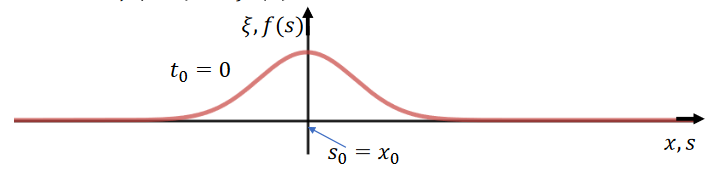
\includegraphics[width=0.8\textwidth]{screenshots/2024-03-12-11-47-01.png}
\end{figure}
Se guardo l'onda in un istante di tempo successivo l'onda si è spostata verso destra:
\begin{figure}[H]
	\centering
	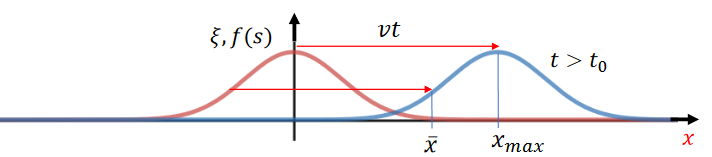
\includegraphics[width=0.8\textwidth]{screenshots/2024-03-12-11-48-57.png}
\end{figure}
Il massimo si può trovare sempre ponendo \(s=0 \rightsquigarrow x_{max} - vt = 0 \rightsquigarrow x_{max} = vt  \). Il massimo si propaga con un'equazione lineare! Non accelera. La forma dell'onda non varia, quindi ogni punto della curva si sposta verso destra con velocità \(v\): \(s = \overline{s} \rightsquigarrow x-vt = \overline{s} \rightsquigarrow \overline{x} = \overline{s} + vt \). Queste considerazioni valgono per qualsiasi onda progressiva.

Le onde meccaniche si descrivono sempre nel sistema di riferimento S in cui il mezzo è fermo (è un SdR privilegiato). Se mi muovo in un sistema di riferimento S' con velocità \(v\) verso destra la funzione \(\xi \) non dipende più dal tempo: l'onda appare ferma. Tuttavia non risolve più l'equazione di D'Alembert (non compaiono derivate seconde rispetto al tempo)! Per studiare le onde devo fare attenzione al sistema di riferimento e pormi in quello privilegiato.

\subsection{Velocità di un'onda}

Il parametro \(v = \sqrt{\frac{T}{\mu }} \) rappresenta quindi la velocità apparente di ogni punto dell'onda. Su corde leggere e sottili (\(\mu \) piccolo) le velocità sono grandi. Su corde grandi e spesse (\(\mu \) grande) le velocità sono piccole. Maggiore è la tensione, maggiore è la velocità.

\subsection{Sovrapposizione di onde}

Le onde possono urtarsi, ma la loro forma non cambia. Facciamo l'esempio di un'onda regressiva e una progressiva:
\begin{figure}[H]
	\centering
	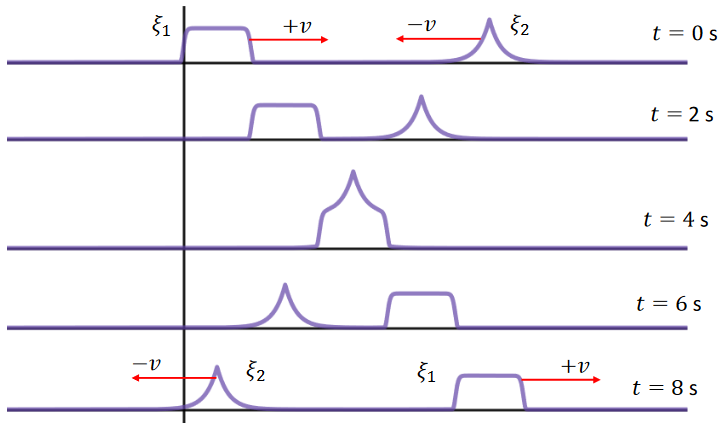
\includegraphics[width=0.6\textwidth]{screenshots/2024-03-12-12-02-37.png}
\end{figure}

\section{Onde armoniche}

Consideriamo una corda elastica tesa, vincolata nella posizione \(x=0\) (detta semi corda). Applichiamo una perturbazione nota sul primo punto della corda: \(\xi (0,t) = -A \sin (\omega t)\) con \(t>0\). 
\begin{figure}[H]
	\centering
	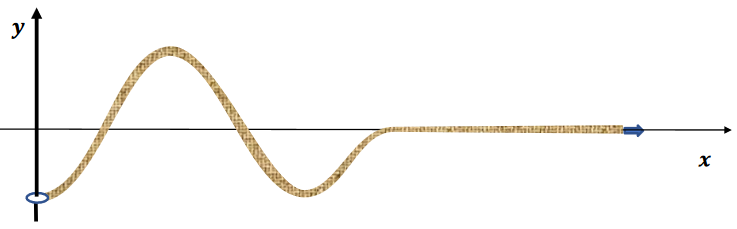
\includegraphics[width=0.8\textwidth]{screenshots/2024-03-12-12-19-43.png}
\end{figure}
Per la forma della corda, \(x_0 = 0\) è sorgente di onde progressive: \(\xi (x,t) = f(x-vt)\). Per \(t>0\) \(\xi (0,t_0) = -A \sin (\omega t_0) = f(x_0 - vt_0) = f(x-vt) = f(s)\). Di conseguenza, \(s=0-vt_0=x-vt \rightsquigarrow t_0 = t-\frac{x}{v} \rightsquigarrow t= t_0 + \frac{x}{v}\). \(\frac{x}{v}\) è il tempo che impiega la perturbazione che avviene al tempo \(t_0\) nel punto \(x_0\) a raggiungere il punto a coordinata x.
\begin{figure}[H]
	\centering
	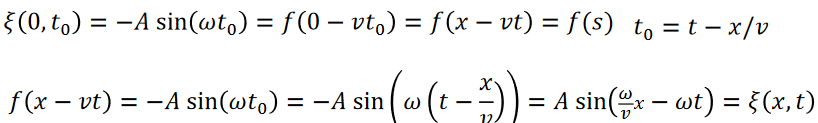
\includegraphics[width=0.8\textwidth]{screenshots/2024-03-12-12-28-56.png}
\end{figure}
I pezzi della corda si mettono progressivamente in moto.

\begin{definition}
	[Numero d'onda]
	Si definisce numero d'onda
	\[
		k = \frac{\omega }{v}
	\]
\end{definition}

L'onda su corda si scrive quindi \(\xi (x,t) = A \sin (kx - \omega t)\). Le onde di questo tipo risolvono l'equazione di D'Alembert e si dicono onde armoniche o monocromatiche (per la loro correlazione con le bande ottiche della luce):
\begin{itemize}
	\item \(\xi (x,t) = A \sin (kx \mp \omega t)\)
	\item \(\xi (x,t) = A \cos (kx \mp \omega t)\)  
\end{itemize}
\begin{figure}[H]
	\centering
	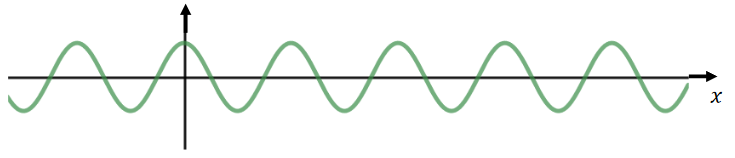
\includegraphics[width=0.8\textwidth]{screenshots/2024-03-12-12-33-41.png}
\end{figure}
Ogni punto dell'onda si muove con velocità \(v\).
\begin{definition}
	[Velocità di fase]
	Si definisce velocità di fase
	\[
		v_f = \frac{\omega }{k}
	\]
	Essa coincide con il parametro \(v\) dell'equazione di D'Alembert.
\end{definition}
Se consideriamo unicamente quello che avviene in un punto di ascissa fissata \(x=\overline{x} \), notiamo che il moto è armonico di periodo \(T_p = \frac{2\pi }{\omega }\). N.B.: i punti della corda si muovono con lo stesso periodo dell'oscillazione della sorgente! È una conseguenza generale: le caratteristiche temporali delle onde sono le stesse in ogni punto dello spazio e dipendono esclusivamente dalla sorgente.

Allo stesso modo possiamo studiare quello che avviene a un istante fissato di tempo: \(t=\overline{t} \). Anche in questo caso si presenta una periodicità, tuttavia è una periodicità spaziale. \(k \lambda = 2\pi \rightsquigarrow \lambda = \frac{2\pi }{k} \rightsquigarrow \lambda = \frac{2 \pi }{\omega } v\). La differenza rispetto a quanto trovato per la periodicità temporale è che in questo caso il valore trovato dipende dalla velocità, che può dipendere dalla posizione nello spazio! \(\lambda \) è detta lunghezza d'onda. La relazione fra \(\lambda \) e T è la seguente:
\begin{definition}
	[Lunghezza d'onda]
\[
	\lambda = \frac{2 \pi }{k}= \frac{2\pi }{\omega }v= vT_p
\]
\end{definition}

\subsection{Utilizzo delle onde armoniche}

L'importanza delle onde armoniche sta nel fatto che per ogni onda armonica ho sempre lo stesso tempo di propagazione. Quindi posso studiare anche fenomeni descritti da onde complicate, come quelle analizzabili con la serie di Fourier. Consideriamo una sollecitazione periodica dell'origine descritta dalla funzione \(f(T)\). Pongo \(\omega _0 = \frac{2\pi }{T}\).
\begin{figure}[H]
	\centering
	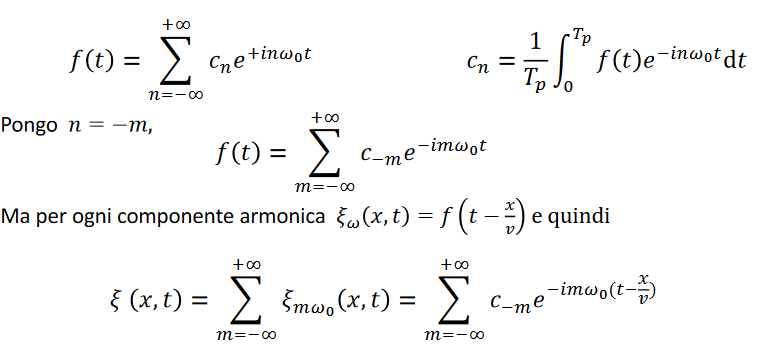
\includegraphics[width=0.8\textwidth]{screenshots/2024-03-12-12-49-14.png}
	\caption{Abbiamo fatto il cambiamento \(n=-m\) perché nelle onde vogliamo sempre avere \(i(kx - \omega t)\).  }
\end{figure}
Cambiando il nome di m in n e ponendo \(\omega _n = n \omega _0, k_n = n \omega _0 / v\). L'onda progressiva si scrive come somma di onde armoniche:
\[
	\xi (x,t) = \sum_{n=-\infty }^{\infty} c^{\prime}_n e^{i(k_n x - \omega _n t)}
\]
Una singola onda armonica si muove con velocità data da \(v_n = \omega_n / k_n\). Quanto fatto si può generalizzare a un caso in cui le onde sono sia regressive che progressive:
\[
	\xi (x,t) = \sum_{n=-\infty }^{\infty} [c_n e^{i(k_n x - \omega _n t)} + d_n e^{i(k_n x + \omega _n t)}]
\]
La potenza di quello che abbiamo appena fatto è che possiamo analizzare qualsiasi segnale periodico in partenza. Si può addirittura generalizzare con l'utilizzo della trasformata di Fourier al posto della serie di Fourier se il segnale di partenza NON è periodico.